\documentclass[tikz,border=8pt]{standalone}

\usepackage[T1]{fontenc}
\usepackage{lmodern}
\usepackage{tikz}
\usetikzlibrary{
    positioning,
    fit,
    arrows.meta,
    shapes.geometric,
    shapes.misc,
    calc
}

\begin{document}
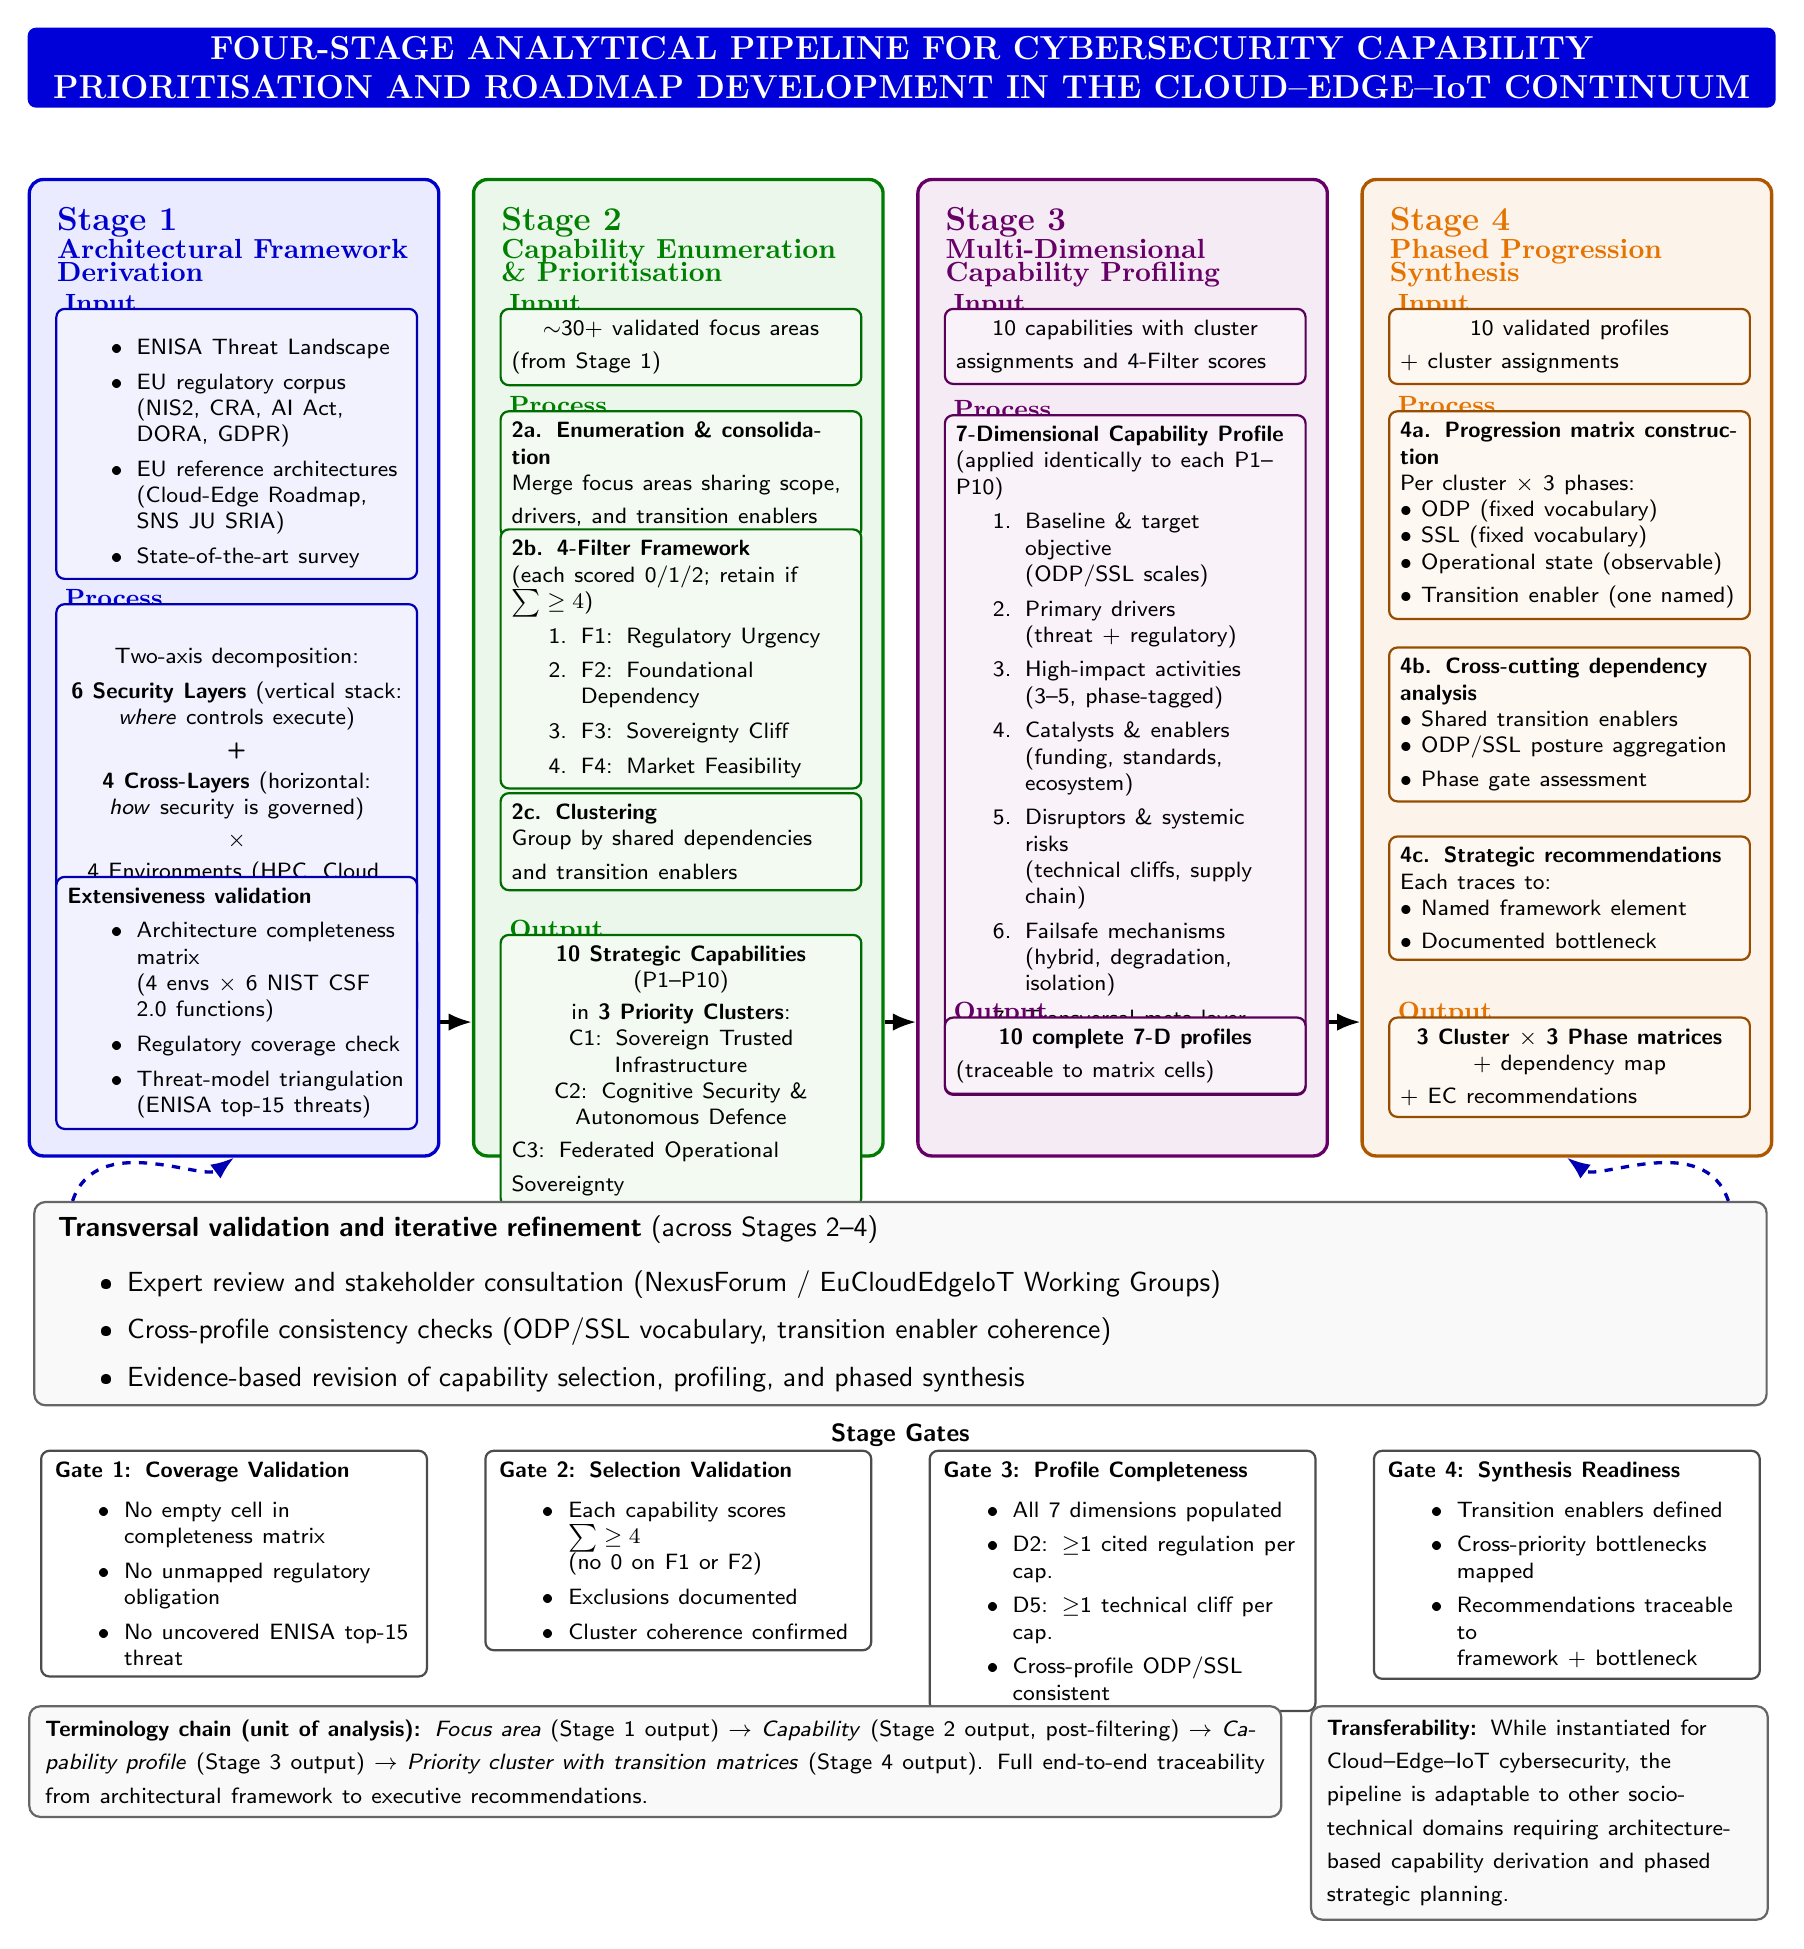
\begin{tikzpicture}[
    font=\sffamily,
    >=Latex,
    node distance=6mm and 7mm,
    stage/.style={
        draw=#1!80!black,
        fill=#1!8,
        rounded corners=5pt,
        very thick,
        minimum width=5.2cm,
        minimum height=12.4cm,
        inner sep=6pt,
        align=left
    },
    smallbox/.style={
        draw=#1!70!black,
        fill=#1!5,
        rounded corners=3pt,
        thick,
        align=left,
        inner sep=4pt
    },
    titlebox/.style={
        fill=blue!85!black,
        text=white,
        rounded corners=3pt,
        minimum height=1cm,
        minimum width=22.2cm,
        align=center,
        font=\bfseries\large
    },
    flow/.style={->, very thick, draw=black},
    vloop/.style={->, very thick, dashed, draw=blue!70!black},
    gate/.style={
        draw=black!70,
        fill=white,
        rounded corners=3pt,
        thick,
        minimum width=4.9cm,
        minimum height=2.1cm,
        text width=4.55cm,
        inner sep=4pt,
        align=left
    },
    legendbox/.style={
        draw=black!60,
        fill=gray!5,
        rounded corners=4pt,
        thick,
        inner sep=5pt,
        align=left
    }
]

% -------------------------------------------------
% Title
% -------------------------------------------------
\node[titlebox] (title) at (11.1,16.5)
{FOUR-STAGE ANALYTICAL PIPELINE FOR CYBERSECURITY CAPABILITY\\
PRIORITISATION AND ROADMAP DEVELOPMENT IN THE CLOUD--EDGE--IoT CONTINUUM};

% -------------------------------------------------
% Stage columns
% -------------------------------------------------
\node[stage=blue, anchor=north west] (s1) at (0,15.1) {};
\node[stage=green!60!black, anchor=north west] (s2) at ($(s1.north east)+(0.4,0)$) {};
\node[stage=violet, anchor=north west] (s3) at ($(s2.north east)+(0.4,0)$) {};
\node[stage=orange!85!black, anchor=north west] (s4) at ($(s3.north east)+(0.4,0)$) {};

% Stage headers
\node[anchor=north west, font=\bfseries\large, text=blue!80!black] at ($(s1.north west)+(0.25,-0.25)$)
{Stage 1};
\node[anchor=north west, font=\bfseries, text=blue!80!black] at ($(s1.north west)+(0.25,-0.65)$)
{Architectural Framework};
\node[anchor=north west, font=\bfseries, text=blue!80!black] at ($(s1.north west)+(0.25,-0.95)$)
{Derivation};

\node[anchor=north west, font=\bfseries\large, text=green!50!black] at ($(s2.north west)+(0.25,-0.25)$)
{Stage 2};
\node[anchor=north west, font=\bfseries, text=green!50!black] at ($(s2.north west)+(0.25,-0.65)$)
{Capability Enumeration};
\node[anchor=north west, font=\bfseries, text=green!50!black] at ($(s2.north west)+(0.25,-0.95)$)
{\& Prioritisation};

\node[anchor=north west, font=\bfseries\large, text=violet!80!black] at ($(s3.north west)+(0.25,-0.25)$)
{Stage 3};
\node[anchor=north west, font=\bfseries, text=violet!80!black] at ($(s3.north west)+(0.25,-0.65)$)
{Multi-Dimensional};
\node[anchor=north west, font=\bfseries, text=violet!80!black] at ($(s3.north west)+(0.25,-0.95)$)
{Capability Profiling};

\node[anchor=north west, font=\bfseries\large, text=orange!90!black] at ($(s4.north west)+(0.25,-0.25)$)
{Stage 4};
\node[anchor=north west, font=\bfseries, text=orange!90!black] at ($(s4.north west)+(0.25,-0.65)$)
{Phased Progression};
\node[anchor=north west, font=\bfseries, text=orange!90!black] at ($(s4.north west)+(0.25,-0.95)$)
{Synthesis};

% -------------------------------------------------
% Stage 1
% -------------------------------------------------
\node[anchor=north west, font=\bfseries\small, text=blue!80!black] at ($(s1.north west)+(0.35,-1.35)$) {Input};

\node[smallbox=blue, text width=4.3cm, anchor=north west] (s1in) at ($(s1.north west)+(0.35,-1.65)$)
{\footnotesize
\begin{itemize}\setlength\itemsep{1pt}
\item ENISA Threat Landscape
\item EU regulatory corpus\\(NIS2, CRA, AI Act, DORA, GDPR)
\item EU reference architectures\\(Cloud-Edge Roadmap, SNS JU SRIA)
\item State-of-the-art survey
\end{itemize}};

\node[anchor=north west, font=\bfseries\small, text=blue!80!black] at ($(s1.north west)+(0.35,-5.1)$) {Process};

\node[smallbox=blue, text width=4.3cm, anchor=north west] (s1proc) at ($(s1.north west)+(0.35,-5.4)$)
{\footnotesize
\begin{center}
Two-axis decomposition:\\[3pt]
\textbf{6 Security Layers} (vertical stack:\\
\textit{where} controls execute)\\[2pt]
\textbf{+}\\[2pt]
\textbf{4 Cross-Layers} (horizontal:\\
\textit{how} security is governed)\\[2pt]
\textbf{$\times$}\\[2pt]
4 Environments (HPC, Cloud, Edge, Device)
\end{center}};

\node[anchor=north west, font=\bfseries\small, text=blue!80!black] at ($(s1.north west)+(0.35,-9.3)$) {Output};

\node[smallbox=blue, text width=4.3cm, anchor=north west] (s1out) at ($(s1.north west)+(0.35,-9.6)$)
{\footnotesize\centering
\textbf{$\sim$30+ named focus areas}\\[2pt]
each with Layer/CL identifier};

\node[smallbox=blue, text width=4.3cm, anchor=south west] (s1val) at ($(s1.south west)+(0.35,0.35)$)
{\footnotesize\textbf{Extensiveness validation}
\begin{itemize}\setlength\itemsep{1pt}
\item Architecture completeness matrix\\(4 envs $\times$ 6 NIST CSF 2.0 functions)
\item Regulatory coverage check
\item Threat-model triangulation\\(ENISA top-15 threats)
\end{itemize}};

% -------------------------------------------------
% Stage 2
% -------------------------------------------------
\node[anchor=north west, font=\bfseries\small, text=green!50!black] at ($(s2.north west)+(0.35,-1.35)$) {Input};

\node[smallbox=green!60!black, text width=4.3cm, anchor=north west] (s2in) at ($(s2.north west)+(0.35,-1.65)$)
{\footnotesize\centering $\sim$30+ validated focus areas\\(from Stage 1)};

\node[anchor=north west, font=\bfseries\small, text=green!50!black] at ($(s2.north west)+(0.35,-2.65)$) {Process};

\node[smallbox=green!60!black, text width=4.3cm, anchor=north west] (s2enum) at ($(s2.north west)+(0.35,-2.95)$)
{\footnotesize\textbf{2a. Enumeration \& consolidation}\\
Merge focus areas sharing scope,\\
drivers, and transition enablers};

\node[smallbox=green!60!black, text width=4.3cm, anchor=north west] (s2filter) at ($(s2.north west)+(0.35,-4.45)$)
{\footnotesize\textbf{2b. 4-Filter Framework}\\(each scored 0/1/2; retain if $\sum \geq 4$)
\begin{enumerate}\setlength\itemsep{1pt}
\item F1: Regulatory Urgency
\item F2: Foundational Dependency
\item F3: Sovereignty Cliff
\item F4: Market Feasibility
\end{enumerate}};

\node[smallbox=green!60!black, text width=4.3cm, anchor=north west] (s2cluster) at ($(s2.north west)+(0.35,-7.8)$)
{\footnotesize\textbf{2c. Clustering}\\
Group by shared dependencies\\and transition enablers};

\node[anchor=north west, font=\bfseries\small, text=green!50!black] at ($(s2.north west)+(0.35,-9.3)$) {Output};

\node[smallbox=green!60!black, text width=4.3cm, anchor=north west] (s2out1) at ($(s2.north west)+(0.35,-9.6)$)
{\footnotesize\centering \textbf{10 Strategic Capabilities} (P1--P10)\\[2pt]
in \textbf{3 Priority Clusters}:\\
C1: Sovereign Trusted Infrastructure\\
C2: Cognitive Security \& Autonomous Defence\\
C3: Federated Operational Sovereignty};

% -------------------------------------------------
% Stage 3
% -------------------------------------------------
\node[anchor=north west, font=\bfseries\small, text=violet!80!black] at ($(s3.north west)+(0.35,-1.35)$) {Input};

\node[smallbox=violet, text width=4.3cm, anchor=north west] (s3in) at ($(s3.north west)+(0.35,-1.65)$)
{\footnotesize\centering 10 capabilities with cluster\\assignments and 4-Filter scores};

\node[anchor=north west, font=\bfseries\small, text=violet!80!black] at ($(s3.north west)+(0.35,-2.7)$) {Process};

\node[smallbox=violet, text width=4.3cm, anchor=north west] (s3profile) at ($(s3.north west)+(0.35,-3.0)$)
{\footnotesize\textbf{7-Dimensional Capability Profile}\\(applied identically to each P1--P10)
\begin{enumerate}\setlength\itemsep{1pt}
\item Baseline \& target objective\\(ODP/SSL scales)
\item Primary drivers\\(threat + regulatory)
\item High-impact activities\\(3--5, phase-tagged)
\item Catalysts \& enablers\\(funding, standards, ecosystem)
\item Disruptors \& systemic risks\\(technical cliffs, supply chain)
\item Failsafe mechanisms\\(hybrid, degradation, isolation)
\item Transversal meta-layer\\(sovereignty, trust, Green IT)
\end{enumerate}};

\node[anchor=north west, font=\bfseries\small, text=violet!80!black] at ($(s3.north west)+(0.35,-10.35)$) {Output};

\node[smallbox=violet, text width=4.3cm, anchor=north west] (s3out) at ($(s3.north west)+(0.35,-10.65)$)
{\footnotesize\centering \textbf{10 complete 7-D profiles}\\
(traceable to matrix cells)};

% -------------------------------------------------
% Stage 4
% -------------------------------------------------
\node[anchor=north west, font=\bfseries\small, text=orange!90!black] at ($(s4.north west)+(0.35,-1.35)$) {Input};

\node[smallbox=orange!85!black, text width=4.3cm, anchor=north west] (s4in) at ($(s4.north west)+(0.35,-1.65)$)
{\footnotesize\centering 10 validated profiles\\+ cluster assignments};

\node[anchor=north west, font=\bfseries\small, text=orange!90!black] at ($(s4.north west)+(0.35,-2.65)$) {Process};

\node[smallbox=orange!85!black, text width=4.3cm, anchor=north west] (s4a) at ($(s4.north west)+(0.35,-2.95)$)
{\footnotesize\textbf{4a. Progression matrix construction}\\
Per cluster $\times$ 3 phases:\\
$\bullet$ ODP (fixed vocabulary)\\
$\bullet$ SSL (fixed vocabulary)\\
$\bullet$ Operational state (observable)\\
$\bullet$ Transition enabler (one named)};

\node[smallbox=orange!85!black, text width=4.3cm, anchor=north west] (s4b) at ($(s4.north west)+(0.35,-5.95)$)
{\footnotesize\textbf{4b. Cross-cutting dependency analysis}\\
$\bullet$ Shared transition enablers\\
$\bullet$ ODP/SSL posture aggregation\\
$\bullet$ Phase gate assessment};

\node[smallbox=orange!85!black, text width=4.3cm, anchor=north west] (s4c) at ($(s4.north west)+(0.35,-8.35)$)
{\footnotesize\textbf{4c. Strategic recommendations}\\
Each traces to:\\
$\bullet$ Named framework element\\
$\bullet$ Documented bottleneck};

\node[anchor=north west, font=\bfseries\small, text=orange!90!black] at ($(s4.north west)+(0.35,-10.35)$) {Output};

\node[smallbox=orange!85!black, text width=4.3cm, anchor=north west] (s4out) at ($(s4.north west)+(0.35,-10.65)$)
{\footnotesize\centering \textbf{3 Cluster $\times$ 3 Phase matrices}\\
+ dependency map\\
+ EC recommendations};

% -------------------------------------------------
% Flows between stages
% -------------------------------------------------
\draw[flow] ($(s1.east)+(0,-4.5)$) -- ($(s2.west)+(0,-4.5)$);
\draw[flow] ($(s2.east)+(0,-4.5)$) -- ($(s3.west)+(0,-4.5)$);
\draw[flow] ($(s3.east)+(0,-4.5)$) -- ($(s4.west)+(0,-4.5)$);

% -------------------------------------------------
% Validation loop
% -------------------------------------------------
\node[legendbox, minimum width=22.0cm, minimum height=2.0cm, text width=21.4cm, anchor=north] (valloop)
    at ($(s1.south)!0.5!(s4.south)+(0,-0.55)$)
{\textbf{Transversal validation and iterative refinement} (across Stages 2--4)
\begin{itemize}\setlength\itemsep{1pt}
\item Expert review and stakeholder consultation (NexusForum / EuCloudEdgeIoT Working Groups)
\item Cross-profile consistency checks (ODP/SSL vocabulary, transition enabler coherence)
\item Evidence-based revision of capability selection, profiling, and phased synthesis
\end{itemize}};

\draw[vloop] ($(valloop.north west)+(0.5,0)$) .. controls +(0.3,0.9) and +(-0.4,-0.3) .. (s1.south);
\draw[vloop] ($(valloop.north east)+(-0.5,0)$) .. controls +(-0.3,0.9) and +(0.4,-0.3) .. (s4.south);

% -------------------------------------------------
% Gates row
% -------------------------------------------------
\node[font=\bfseries\small\sffamily, align=center, anchor=north] (gtitle)
    at ($(valloop.south)+(0,-0.1)$)
    {Stage Gates};

\node[gate, anchor=north] (g1) at ($(s1.south |- valloop.south)+(0,-0.55)$)
{\footnotesize\textbf{Gate 1: Coverage Validation}\\[2pt]
\begin{itemize}\setlength\itemsep{1pt}
\item No empty cell in completeness matrix
\item No unmapped regulatory obligation
\item No uncovered ENISA top-15 threat
\end{itemize}};

\node[gate, anchor=north] (g2) at ($(s2.south |- valloop.south)+(0,-0.55)$)
{\footnotesize\textbf{Gate 2: Selection Validation}\\[2pt]
\begin{itemize}\setlength\itemsep{1pt}
\item Each capability scores $\sum \geq 4$\\(no 0 on F1 or F2)
\item Exclusions documented
\item Cluster coherence confirmed
\end{itemize}};

\node[gate, anchor=north] (g3) at ($(s3.south |- valloop.south)+(0,-0.55)$)
{\footnotesize\textbf{Gate 3: Profile Completeness}\\[2pt]
\begin{itemize}\setlength\itemsep{1pt}
\item All 7 dimensions populated
\item D2: $\geq$1 cited regulation per cap.
\item D5: $\geq$1 technical cliff per cap.
\item Cross-profile ODP/SSL consistent
\end{itemize}};

\node[gate, anchor=north] (g4) at ($(s4.south |- valloop.south)+(0,-0.55)$)
{\footnotesize\textbf{Gate 4: Synthesis Readiness}\\[2pt]
\begin{itemize}\setlength\itemsep{1pt}
\item Transition enablers defined
\item Cross-priority bottlenecks mapped
\item Recommendations traceable to\\framework + bottleneck
\end{itemize}};

% -------------------------------------------------
% Bottom: terminology chain + transferability
% -------------------------------------------------
\node[legendbox, minimum width=15.9cm, minimum height=1.4cm, text width=15.5cm, anchor=north west] (unit)
    at ($(g1.south west)+(-0.15,-0.35)$)
{\footnotesize\textbf{Terminology chain (unit of analysis):}
\textit{Focus area} (Stage 1 output) $\rightarrow$ \textit{Capability} (Stage 2 output, post-filtering) $\rightarrow$
\textit{Capability profile} (Stage 3 output) $\rightarrow$ \textit{Priority cluster with transition matrices} (Stage 4 output).
Full end-to-end traceability from architectural framework to executive recommendations.};

\node[legendbox, minimum width=5.8cm, minimum height=1.4cm, text width=5.4cm, anchor=north west] (gen)
at ($(unit.north east)+(0.35,0)$)
{\footnotesize\textbf{Transferability:}
While instantiated for Cloud--Edge--IoT cybersecurity, the pipeline is adaptable to other socio-technical domains requiring architecture-based capability derivation and phased strategic planning.};

\end{tikzpicture}
\end{document}